\begin{figure}[tbh]
    \centering
    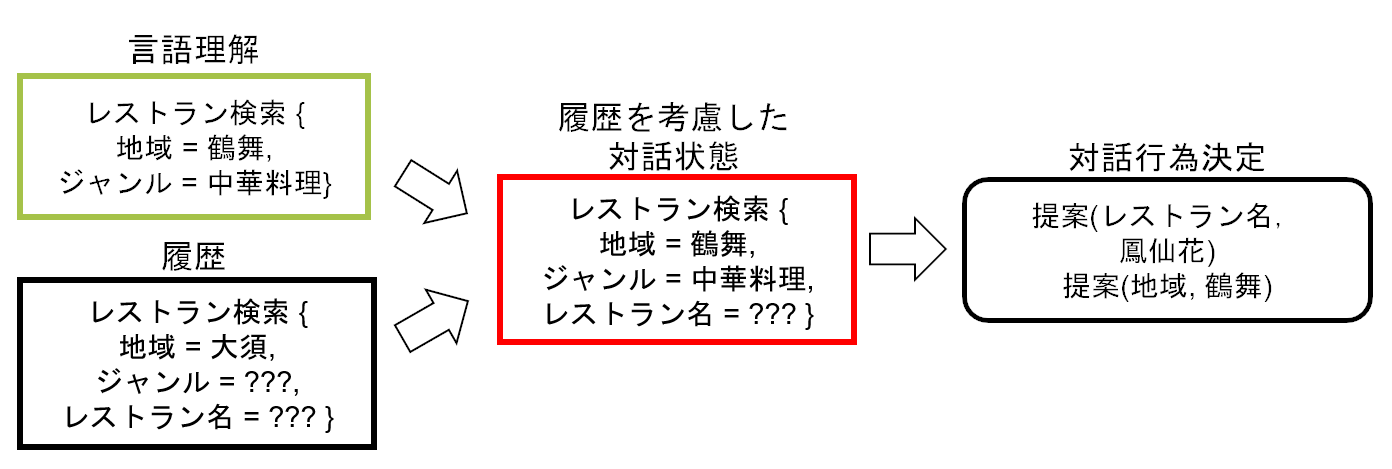
\includegraphics[width=15cm]{chapter2/dst2.eps}
    \caption{対話管理部の処理の流れ}
    \label{fig:dst}
\end{figure}

対話システムにおける対話状態追跡は,図\ref{fig:taiwasystem}に示した通り対話管理部の機能の1つである.対話管理部の処理は図\ref{fig:dst}のような流れになっている.対話状態追跡は言語理解の結果と履歴を考慮して,対話状態を出力する.この図において,履歴は一例として前のターンの対話状態を用いている.対話状態はレストラン検索などといった目的と,スロットと値の組を用いた辞書形式で表現される.システムは対話状態にある目的を達成するために必要なスロットを埋めていく作業を行う.つまり,対話状態追跡は対話状態のスロット値を言語理解の結果から得たスロット値候補に変更するか否かを判断する役割を担う.また,対話行為決定では対話状態の不足している情報を検出して,目的達成に向けて必要なシステムの対話行為を選択する.
\par
システムは対話状態を見て次の行動を決めるため,対話状態追跡が対話状態の推定を誤ると,ユーザの要求にそぐわない対話を行うことになる.ゆえに対話状態追跡はタスク指向型対話システムにとって重要な要素である.